\documentclass[conference]{IEEEtran}
\IEEEoverridecommandlockouts

\usepackage[utf8]{inputenc}
\usepackage[vietnamese]{babel}
\usepackage{cite}
\usepackage{amsmath,amssymb,amsfonts}
\usepackage{graphicx}
\usepackage{textcomp}
\usepackage{xcolor}
\usepackage{booktabs}
\usepackage{hyperref}
\usepackage{listings}
\usepackage{algorithm}
\usepackage{algpseudocode}
\usepackage{multirow}
\usepackage{array}
\usepackage{url}

\lstset{
  basicstyle=\ttfamily\footnotesize,
  breaklines=true,
  frame=single,
  numbers=left,
  numberstyle=\tiny,
}

\def\BibTeX{{\rm B\kern-.05em{\sc i\kern-.025em b}\kern-.08em
    T\kern-.1667em\lower.7ex\hbox{E}\kern-.125emX}}

\begin{document}

\title{Hệ Thống Dự Đoán Churn Người Dùng Theo Thời Gian Thực:\\
Một Pipeline MLOps End-to-End Trên Nền Tảng GCP}

\author{
  \IEEEauthorblockN{Nguyễn Phương Trí}
  \IEEEauthorblockA{
    \textit{Học viên Kỹ thuật Phần mềm} \\
    ptrnghieu@gmail.com
  }
}

\maketitle

%──────────────────────────────────────────────────────────────────────────────
\begin{abstract}
Bài báo này trình bày thiết kế và triển khai một hệ thống MLOps end-to-end
nhằm dự đoán khả năng rời bỏ dịch vụ (churn) của người dùng nền tảng phát
nhạc trực tuyến KKBox. Hệ thống tích hợp pipeline xử lý dữ liệu streaming
qua Apache Kafka, mô hình phân loại XGBoost được huấn luyện với chiến lược
out-of-time validation, và một API phục vụ trực tuyến sử dụng FastAPI cùng
Feast Feature Store trên Google Cloud Platform (GCP). Điểm đặc trưng của
giải pháp là cơ chế \emph{historical playback}: dữ liệu năm 2017 được phát
lại từng ngày qua Kafka để giả lập môi trường streaming thực tế, kết hợp với
kỹ thuật tích lũy đặc trưng liên tục (\emph{cumulative feature aggregation})
nhằm duy trì nhất quán phân phối giữa tập huấn luyện và môi trường sản xuất.
Mô hình đạt AUC-ROC = 0,8924 và AUC-PR = 0,5044 trên tập kiểm tra
out-of-time. Hệ thống được triển khai trên GCE VM với nginx reverse proxy,
systemd service, và React dashboard tích hợp trực tiếp trong API server.
\end{abstract}

\begin{IEEEkeywords}
churn prediction, MLOps, Apache Kafka, XGBoost, SHAP, Feature Store,
streaming simulation, GCP, FastAPI
\end{IEEEkeywords}

%──────────────────────────────────────────────────────────────────────────────
\section{Giới Thiệu}

Dự đoán churn (customer churn prediction) là bài toán phân loại nhị phân quan
trọng trong các nền tảng dịch vụ theo mô hình đăng ký (subscription-based
services): liệu một người dùng có hủy đăng ký trong chu kỳ tiếp theo hay
không~\cite{verbeke2012new}. Chi phí giữ chân một khách hàng hiện tại thường
thấp hơn đáng kể so với chi phí thu hút khách hàng mới, vì vậy việc phát hiện
sớm nguy cơ churn cho phép doanh nghiệp can thiệp kịp thời bằng các chương
trình khuyến mãi hoặc cải thiện trải nghiệm người dùng~\cite{hadden2007computer}.

KKBox là nền tảng phát nhạc trực tuyến lớn tại Đài Loan và Đông Nam Á, với
hàng triệu người dùng đăng ký theo tháng. Dữ liệu KKBox được công bố tại
Kaggle WSDM Cup 2018~\cite{wsdm2018} bao gồm lịch sử giao dịch, nhật ký nghe
nhạc, và thông tin thành viên — đủ phong phú để xây dựng các đặc trưng hành
vi người dùng có tính dự đoán cao.

Thách thức chính trong bài toán này không chỉ nằm ở việc xây dựng mô hình
chính xác, mà còn ở khâu vận hành sản xuất: (i)~đặc trưng phải được cập nhật
liên tục khi người dùng tương tác với hệ thống, (ii)~phân phối đặc trưng tại
thời điểm phục vụ (serving time) phải nhất quán với phân phối lúc huấn luyện
để tránh \emph{training-serving skew}, và (iii)~hệ thống phải có khả năng xử
lý dự đoán theo thời gian thực với độ trễ thấp.

Bài báo này đóng góp:
\begin{itemize}
  \item Thiết kế pipeline MLOps end-to-end tích hợp Kafka streaming, BigQuery,
        Feast Feature Store, và FastAPI trên GCP.
  \item Cơ chế \emph{cumulative feature aggregation}: đặc trưng streaming được
        tích lũy dần lên baseline snapshot, đảm bảo phân phối nhất quán với
        tập huấn luyện.
  \item Chiến lược \emph{cold-start median imputation}: người dùng mới chưa có
        đặc trưng trong Feature Store được điền bằng median population thay vì
        giá trị không (zero imputation), giảm thiểu bias dự đoán.
  \item Công cụ \emph{streaming simulation} cho phép phát lại dữ liệu lịch sử
        theo thời gian thực phục vụ demo và kiểm thử hệ thống.
\end{itemize}

Phần còn lại của bài báo được tổ chức như sau: Phần~\ref{sec:related} tóm tắt
các công trình liên quan. Phần~\ref{sec:arch} mô tả kiến trúc tổng thể.
Phần~\ref{sec:data} trình bày kỹ thuật xây dựng đặc trưng. Phần~\ref{sec:model}
mô tả mô hình và quy trình huấn luyện. Phần~\ref{sec:serving} trình bày hệ
thống phục vụ. Phần~\ref{sec:results} phân tích kết quả thực nghiệm.
Phần~\ref{sec:conclusion} kết luận.

%──────────────────────────────────────────────────────────────────────────────
\section{Công Trình Liên Quan}
\label{sec:related}

\subsection{Mô hình dự đoán churn}

Các phương pháp học máy đã được áp dụng rộng rãi cho bài toán churn
prediction. Logistic Regression và Decision Tree là các baseline phổ biến do
khả năng diễn giải cao~\cite{verbeke2012new}. Random Forest và Gradient
Boosted Trees (GBT) như XGBoost~\cite{chen2016xgboost} và LightGBM thường đạt
kết quả tốt hơn trên dữ liệu dạng bảng nhờ khả năng xử lý phi tuyến tính và
tương tác đặc trưng. Mạng nơ-ron hồi quy (LSTM, GRU) được đề xuất cho chuỗi
thời gian hành vi người dùng~\cite{graves2013generating}, nhưng đòi hỏi lượng
dữ liệu lớn và chi phí huấn luyện cao.

Trong bối cảnh KKBox, nghiên cứu của Yu et al.~\cite{yu2018} (giải nhì WSDM
Cup 2018) sử dụng LightGBM với các đặc trưng thống kê tổng hợp từ lịch sử
giao dịch và nhật ký nghe nhạc, đạt AUC-ROC $\approx$ 0,91 trên leaderboard
công khai. Tuy nhiên, các giải pháp thi đấu thường tập trung vào tối ưu hóa
metric mà không quan tâm đến khả năng triển khai thực tế.

\subsection{MLOps và Feature Store}

MLOps~\cite{kreuzberger2023machine} là tập hợp các nguyên tắc và công cụ kết
hợp Machine Learning với DevOps, nhằm tự động hóa và chuẩn hóa vòng đời mô
hình từ phát triển đến sản xuất. Feature Store là thành phần quan trọng trong
kiến trúc MLOps hiện đại, đóng vai trò trung gian lưu trữ và phục vụ đặc
trưng cho cả quá trình huấn luyện (offline) và dự đoán (online)~\cite{feast}.
Feast~\cite{feast} là một Feature Store mã nguồn mở hỗ trợ nhiều backend lưu
trữ, bao gồm BigQuery (offline) và Redis (online).

\subsection{Streaming và dự đoán thời gian thực}

Apache Kafka~\cite{kafka} là nền tảng streaming phân tán được sử dụng rộng
rãi trong các hệ thống xử lý sự kiện theo thời gian thực. Kết hợp Kafka với
Feature Store cho phép cập nhật đặc trưng người dùng liên tục khi có dữ liệu
mới, duy trì tính nhất quán giữa trạng thái người dùng và dự đoán của
mô hình~\cite{realtime_ml}.

%──────────────────────────────────────────────────────────────────────────────
\section{Kiến Trúc Hệ Thống}
\label{sec:arch}

\begin{figure}[htbp]
  \centering
  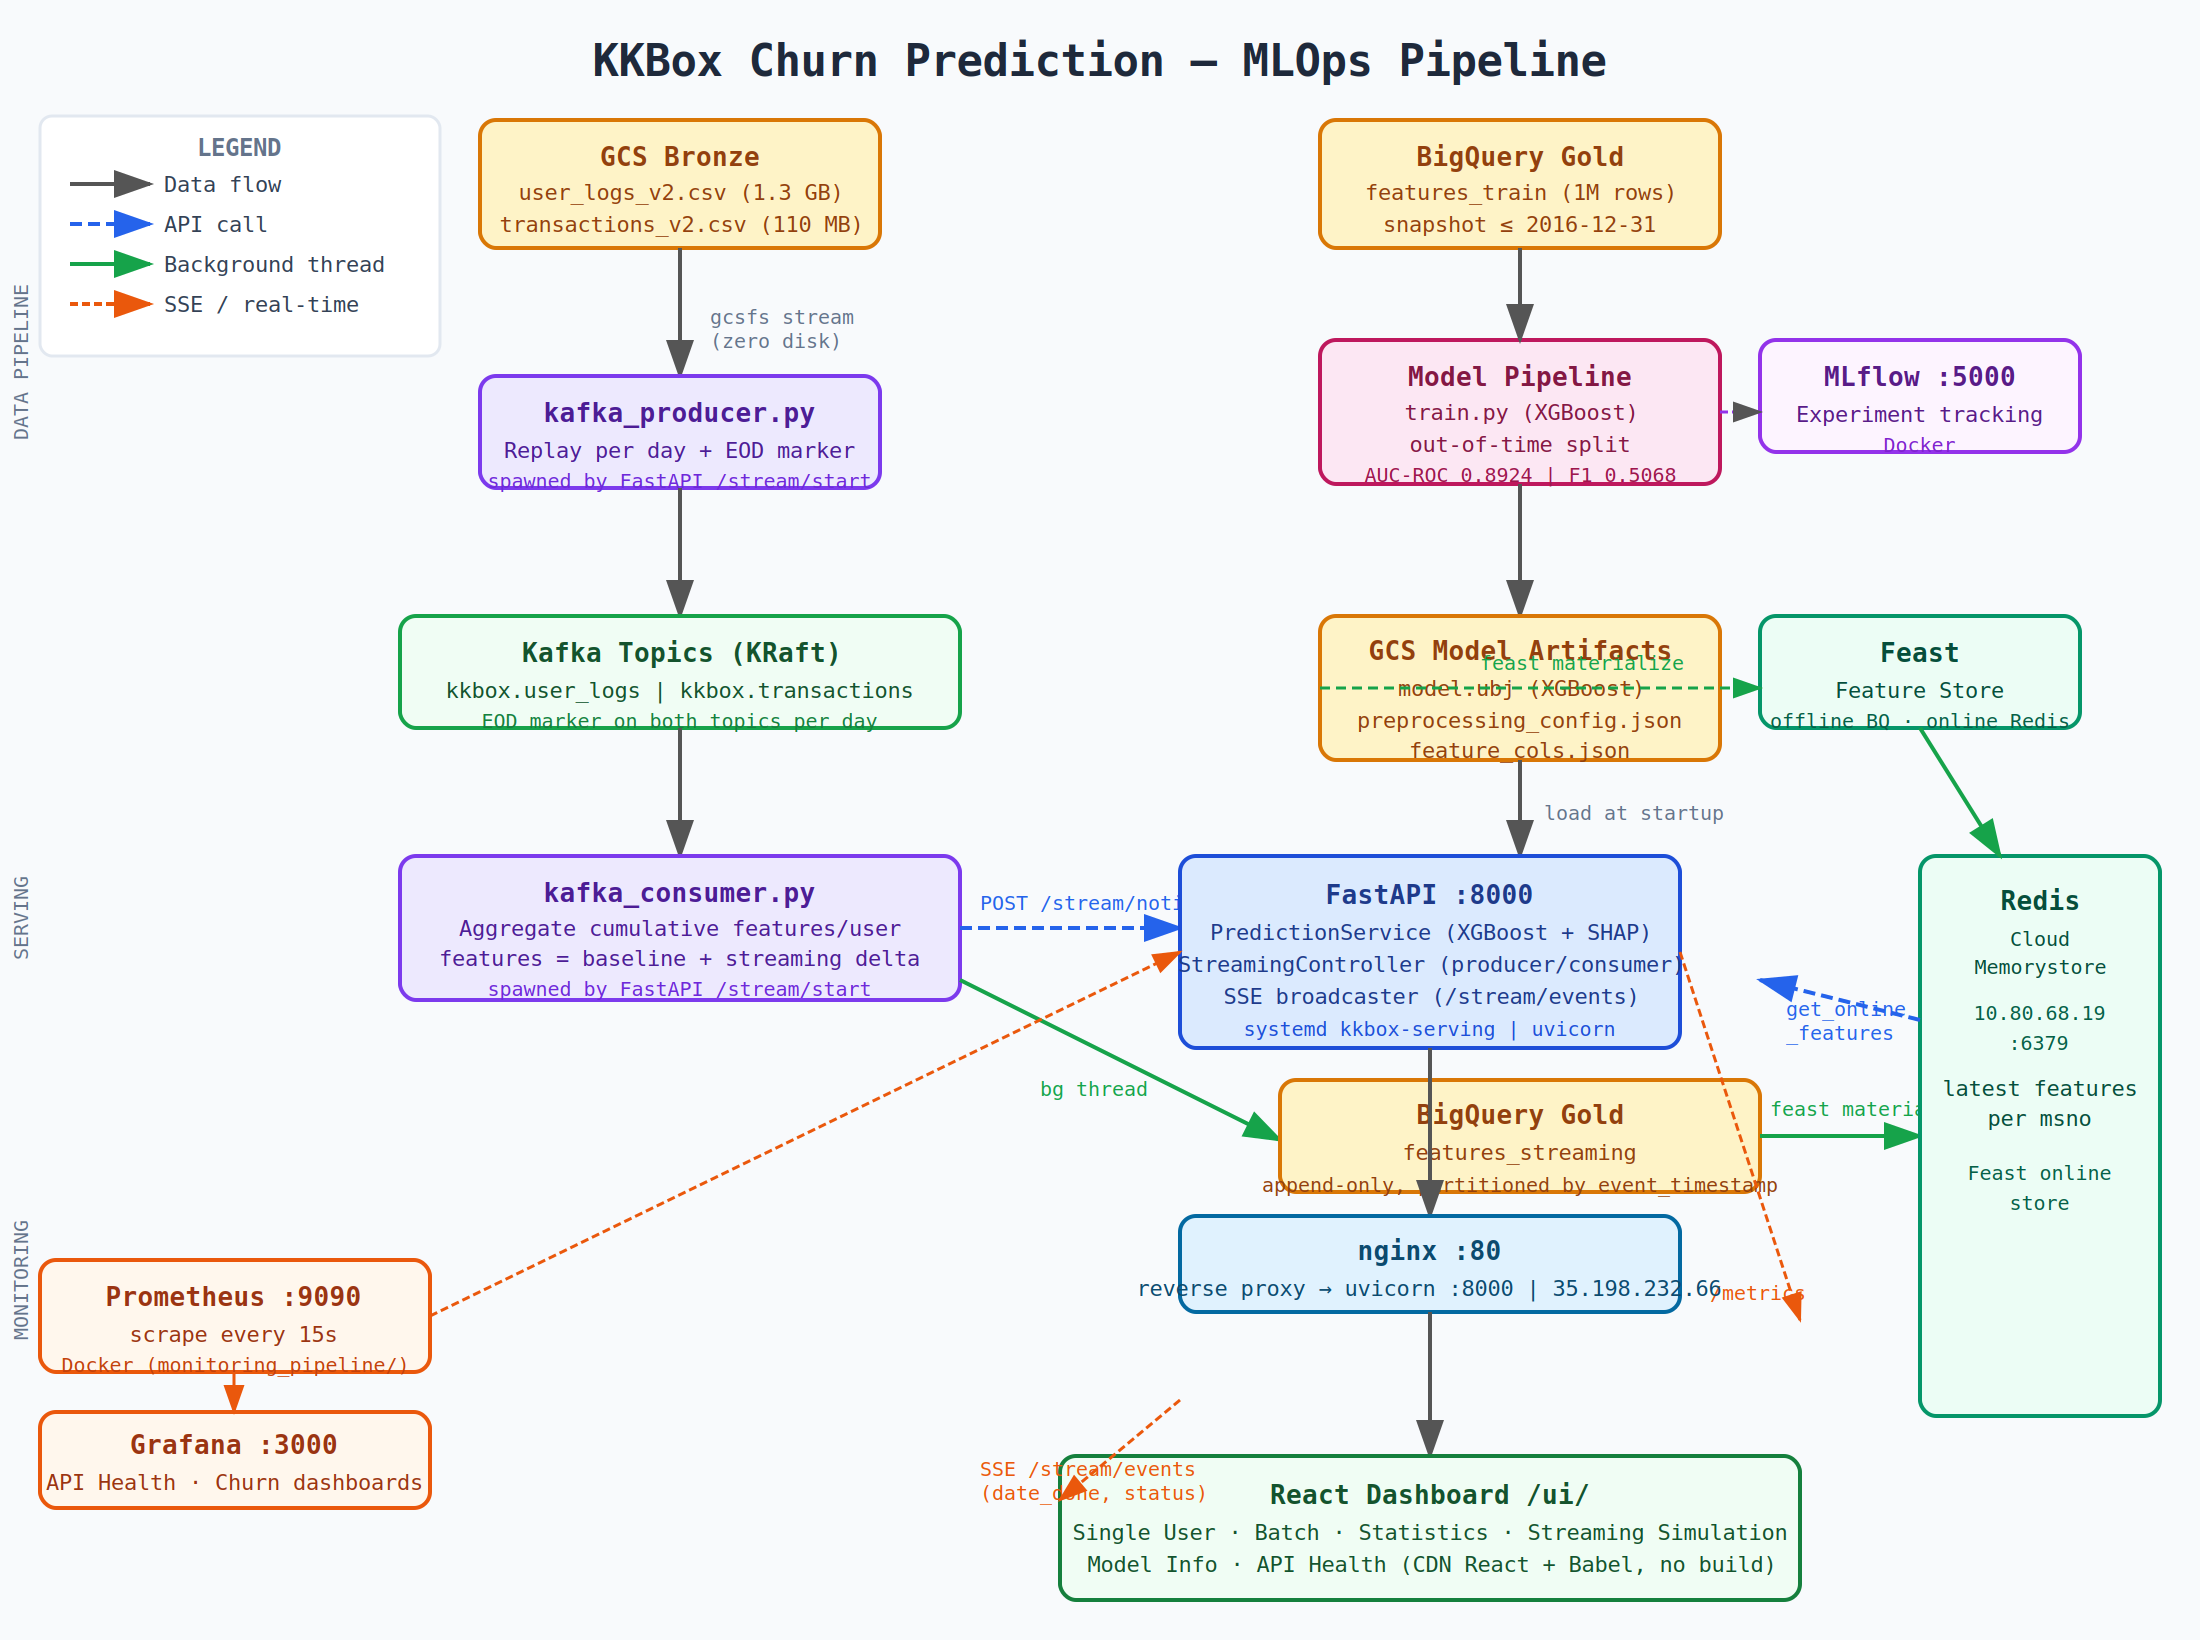
\includegraphics[width=\columnwidth]{pipeline.png}
  \caption{Kiến trúc tổng thể hệ thống KKBox Churn Prediction MLOps.}
  \label{fig:arch}
\end{figure}

Hình~\ref{fig:arch} mô tả kiến trúc tổng thể. Hệ thống gồm bốn pipeline
chính:

\textbf{Data Pipeline} xử lý luồng dữ liệu từ GCS Bronze đến BigQuery Gold
và Redis thông qua Kafka. \textbf{Model Pipeline} huấn luyện mô hình XGBoost
từ BigQuery Gold và lưu artifact lên GCS. \textbf{Serving Pipeline} phục vụ
dự đoán trực tuyến qua FastAPI, đọc đặc trưng từ Redis qua Feast.
\textbf{Monitoring Pipeline} thu thập và hiển thị metrics qua Prometheus và
Grafana.

\subsection{Data Lake Architecture}

Dữ liệu được tổ chức theo kiến trúc Medallion:

\begin{itemize}
  \item \textbf{Bronze}: CSV gốc từ Kaggle lưu trên GCS
        (\texttt{user\_logs.csv} 28,4~GB, \texttt{transactions.csv} 1,6~GB)
        và dữ liệu streaming 2017 (\texttt{user\_logs\_v2.csv} 1,3~GB,
        \texttt{transactions\_v2.csv} 110~MB).
  \item \textbf{Silver}: Parquet sau khi làm sạch, đúc kiểu dữ liệu, và
        khử trùng lặp qua Apache Spark trên Google Dataproc.
  \item \textbf{Gold}: Bảng đặc trưng tổng hợp trên BigQuery
        (\texttt{features\_train} cho huấn luyện,
        \texttt{features\_streaming} cho streaming cập nhật).
\end{itemize}

\subsection{Chiến lược Historical Playback}

Thay vì xây dựng hệ thống streaming thực tế đòi hỏi hạ tầng phức tạp, chúng
tôi sử dụng chiến lược \emph{historical playback}: dữ liệu người dùng năm
2017 (file \texttt{\_v2}) được phát lại tuần tự qua Kafka, mỗi ngày được xử
lý độc lập với độ trễ có thể điều chỉnh. Đây là kỹ thuật phổ biến trong
demo và kiểm thử hệ thống streaming~\cite{realtime_ml}. Chiến lược này cho
phép kiểm chứng toàn bộ pipeline end-to-end mà không cần chờ dữ liệu thực
tế tích lũy.

%──────────────────────────────────────────────────────────────────────────────
\section{Xây Dựng Đặc Trưng}
\label{sec:data}

\subsection{Tập dữ liệu}

Dữ liệu huấn luyện được lấy từ bảng
\texttt{kkbox\_gold.features\_train} trên BigQuery, chứa snapshot đặc trưng
người dùng tính đến ngày 31/12/2016 với 1.082.190 dòng và tỉ lệ churn 10\%.
Mỗi dòng tương ứng với một người dùng duy nhất (entity key: \texttt{msno}).

\subsection{Chiến lược phân chia dữ liệu}

Thay vì phân chia ngẫu nhiên (random split), chúng tôi sử dụng
\textbf{out-of-time split} dựa trên thời điểm đăng ký
(\texttt{registration\_init\_time}):

\begin{equation}
  \text{Train: } \textit{reg\_time} < \text{2016-06-01}
  \quad (\approx 804\text{k dòng})
\end{equation}
\begin{equation}
  \text{Test: } \textit{reg\_time} \geq \text{2016-06-01}
  \quad (\approx 157\text{k dòng})
\end{equation}

Chiến lược này phản ánh thực tế triển khai: mô hình được huấn luyện trên
người dùng đăng ký sớm hơn và dự đoán cho người dùng đăng ký muộn hơn, tránh
data leakage và đánh giá khả năng tổng quát hóa theo thời gian~\cite{oot_split}.

\subsection{Bộ đặc trưng}

18 đặc trưng được xây dựng từ ba nguồn dữ liệu như trong Bảng~\ref{tab:features}.

\begin{table}[htbp]
\caption{Bộ đặc trưng sử dụng trong huấn luyện}
\label{tab:features}
\centering
\begin{tabular}{lll}
\toprule
\textbf{Đặc trưng} & \textbf{Nguồn} & \textbf{Mô tả} \\
\midrule
\texttt{city} & members & Thành phố đăng ký \\
\texttt{bd} & members & Tuổi người dùng \\
\texttt{gender} & members & Giới tính (encoded) \\
\texttt{registered\_via} & members & Kênh đăng ký \\
\midrule
\texttt{total\_transactions} & transactions & Tổng số giao dịch \\
\texttt{total\_amount\_paid} & transactions & Tổng tiền đã thanh toán \\
\texttt{avg\_amount\_paid} & transactions & Trung bình mỗi giao dịch \\
\texttt{auto\_renew\_count} & transactions & Số lần tự động gia hạn \\
\texttt{cancel\_count} & transactions & Số lần hủy gói \\
\midrule
\texttt{total\_log\_days} & user\_logs & Số ngày có hoạt động \\
\texttt{total\_secs} & user\_logs & Tổng giây nghe nhạc \\
\texttt{avg\_daily\_secs} & user\_logs & Trung bình giây/ngày \\
\texttt{total\_num\_25} & user\_logs & Bài nghe được 25\% \\
\texttt{total\_num\_50} & user\_logs & Bài nghe được 50\% \\
\texttt{total\_num\_75} & user\_logs & Bài nghe được 75\% \\
\texttt{total\_num\_985} & user\_logs & Bài nghe được 98,5\% \\
\texttt{total\_num\_100} & user\_logs & Bài nghe hoàn toàn \\
\texttt{total\_num\_unq} & user\_logs & Số bài hát unique \\
\bottomrule
\end{tabular}
\end{table}

\subsection{Cumulative Feature Aggregation}

Trong môi trường streaming, một thách thức quan trọng là duy trì nhất quán
phân phối đặc trưng giữa training và serving. Nếu chỉ sử dụng dữ liệu của
một ngày duy nhất (daily snapshot), các đặc trưng tổng hợp như
\texttt{total\_secs} hay \texttt{total\_transactions} sẽ có phân phối hoàn
toàn khác so với snapshot tích lũy nhiều tháng dùng lúc huấn luyện — gây ra
\emph{training-serving skew} nghiêm trọng.

Chúng tôi giải quyết vấn đề này bằng kỹ thuật \textbf{cumulative feature
aggregation}:

\begin{equation}
  \mathbf{x}_t = \mathbf{x}_{0} + \sum_{d=1}^{t} \Delta\mathbf{x}_d
\end{equation}

trong đó $\mathbf{x}_{0}$ là baseline snapshot từ \texttt{features\_train}
(tính đến 31/12/2016) và $\Delta\mathbf{x}_d$ là delta tổng hợp từ dữ liệu
ngày $d$ trong streaming. Mỗi ngày mới, delta được cộng dồn vào baseline và
ghi lên Redis thông qua Feast, tạo ra vector đặc trưng mới nhất cho từng
người dùng mà có phân phối tương đồng với tập huấn luyện.

\subsection{Cold-start Imputation}

Người dùng mới chưa xuất hiện trong streaming (không có đặc trưng trong
Redis) được xử lý bằng \textbf{population median imputation}: thay vì điền
giá trị 0 (khiến mô hình nhầm tưởng người dùng hoàn toàn không hoạt động),
chúng tôi điền bằng median của từng đặc trưng số tính từ tập huấn luyện:

\begin{equation}
  x_{\text{cold}} = \text{median}(\{x_i : i \in \mathcal{D}_{\text{train}}\})
\end{equation}

Median được tính và lưu vào \texttt{preprocessing\_config.json} trong quá
trình huấn luyện, đảm bảo nhất quán giữa training và serving.

%──────────────────────────────────────────────────────────────────────────────
\section{Mô Hình Học Máy}
\label{sec:model}

\subsection{Lựa chọn mô hình}

Chúng tôi chọn XGBoost~\cite{chen2016xgboost} (Extreme Gradient Boosting) vì
những ưu điểm phù hợp với bài toán:

\begin{itemize}
  \item Hiệu suất cao trên dữ liệu bảng với đặc trưng hỗn hợp (số + phân loại).
  \item Xử lý tốt dữ liệu mất cân bằng lớp thông qua tham số
        \texttt{scale\_pos\_weight}.
  \item Tương thích với SHAP TreeExplainer để giải thích dự đoán theo từng
        đặc trưng.
  \item Tốc độ inference nhanh, phù hợp cho dự đoán trực tuyến.
\end{itemize}

\subsection{Xử lý mất cân bằng lớp}

Dữ liệu có tỉ lệ churn 10\%, gây mất cân bằng lớp đáng kể (imbalanced
classification). Chúng tôi sử dụng tham số \texttt{scale\_pos\_weight}:

\begin{equation}
  \texttt{scale\_pos\_weight} = \frac{|\text{negative}|}{|\text{positive}|}
  = \frac{|\text{không churn}|}{|\text{churn}|} \approx 9{,}0
\end{equation}

Điều này tương đương với việc tăng trọng số cho lớp thiểu số (minority class)
trong hàm loss, giúp mô hình nhạy hơn với người dùng có nguy cơ churn.

\subsection{Siêu tham số}

Bảng~\ref{tab:hyperparams} liệt kê cấu hình mô hình cuối cùng.

\begin{table}[htbp]
\caption{Siêu tham số XGBoost}
\label{tab:hyperparams}
\centering
\begin{tabular}{ll}
\toprule
\textbf{Tham số} & \textbf{Giá trị} \\
\midrule
\texttt{n\_estimators} & 500 \\
\texttt{max\_depth} & 6 \\
\texttt{learning\_rate} & 0,05 \\
\texttt{subsample} & 0,8 \\
\texttt{colsample\_bytree} & 0,8 \\
\texttt{min\_child\_weight} & 10 \\
\texttt{scale\_pos\_weight} & $\approx$ 9,0 \\
\texttt{eval\_metric} & AUC \\
\texttt{early\_stopping\_rounds} & 30 \\
\bottomrule
\end{tabular}
\end{table}

\subsection{Lựa chọn ngưỡng quyết định}

XGBoost trả về xác suất $p \in [0, 1]$. Ngưỡng mặc định $p \geq 0{,}5$ không
tối ưu cho dữ liệu mất cân bằng. Chúng tôi chọn ngưỡng tối đa hóa F1-score
trên tập kiểm tra:

\begin{equation}
  \hat{\tau} = \arg\max_\tau F_1(\tau) = \arg\max_\tau
  \frac{2 \cdot P(\tau) \cdot R(\tau)}{P(\tau) + R(\tau)}
\end{equation}

Kết quả: $\hat{\tau} = 0{,}789$. Ngưỡng mặc định trong serving là $0{,}781$
(có thể điều chỉnh qua biến môi trường \texttt{CHURN\_THRESHOLD} để phù hợp
với chính sách kinh doanh).

\subsection{Theo dõi thực nghiệm với MLflow}

Mỗi lần chạy huấn luyện được log tự động vào MLflow với đầy đủ thông số, số
liệu, và artifact (model, preprocessing config, feature list). Artifact được
lưu đồng thời lên GCS tại đường dẫn cố định để API phục vụ có thể tải mà
không phụ thuộc vào MLflow registry.

\subsection{Giải thích dự đoán với SHAP}

Để tăng tính minh bạch, chúng tôi tích hợp SHAP (SHapley Additive
exPlanations)~\cite{lundberg2017unified}. SHAP TreeExplainer được khởi tạo
một lần khi server khởi động và tái sử dụng cho tất cả request:

\begin{equation}
  \phi_j = \sum_{S \subseteq F \setminus \{j\}} \frac{|S|!(|F|-|S|-1)!}{|F|!}
  \left[ v(S \cup \{j\}) - v(S) \right]
\end{equation}

Top-3 đặc trưng có SHAP value dương lớn nhất (đóng góp tích cực vào nguy cơ
churn) được chuyển đổi thành câu giải thích ngôn ngữ tự nhiên và trả về trong
response API, giúp nhân viên chăm sóc khách hàng hiểu lý do cảnh báo.

%──────────────────────────────────────────────────────────────────────────────
\section{Hệ Thống Phục Vụ}
\label{sec:serving}

\subsection{Data Pipeline Streaming}

\textbf{kafka\_producer.py} đọc trực tiếp từ GCS bằng \texttt{gcsfs} (không
ghi xuống đĩa cục bộ), phát lại dữ liệu từng ngày theo thứ tự thời gian. Sau
khi hoàn thành mỗi ngày, producer gửi EOD marker (\emph{End-of-Day}) lên cả
hai topic \texttt{kkbox.user\_logs} và \texttt{kkbox.transactions}.

\textbf{kafka\_consumer.py} implement một vòng lặp tiêu thụ Kafka với các đặc
điểm kỹ thuật quan trọng:

\begin{enumerate}
  \item \textbf{Lock offset sớm}: Consumer được khởi động trước producer 20
        giây với \texttt{auto\_offset\_reset=latest}, đảm bảo không bỏ sót
        message trong cửa sổ khởi động.
  \item \textbf{Dual EOD tracking}: Flush một ngày chỉ xảy ra khi nhận được
        EOD marker trên \emph{cả hai} topic, tránh flush với dữ liệu chưa
        đầy đủ (race condition).
  \item \textbf{Background thread}: Ghi BigQuery và materialize Feast được
        thực hiện trong background thread qua \texttt{queue.Queue}, không chặn
        consumer loop xử lý ngày tiếp theo.
  \item \textbf{Non-blocking notify}: \texttt{POST /stream/notify} được gửi
        đến FastAPI \emph{trước} khi ghi BQ/Feast, cho phép UI cập nhật ngay
        lập tức.
\end{enumerate}

\begin{algorithm}
\caption{Consumer EOD Flush Logic}
\begin{algorithmic}[1]
\State $eod\_logs \gets \emptyset$, $eod\_txns \gets \emptyset$
\State $flushed \gets \emptyset$
\For{each record from Kafka}
  \If{record is EOD marker for date $d$}
    \State Add $d$ to $eod\_logs$ or $eod\_txns$ (based on topic)
    \If{$d \in eod\_logs$ \textbf{and} $d \in eod\_txns$ \textbf{and} $d \notin flushed$}
      \State \Call{PostNotify}{$d$} \Comment{non-blocking}
      \State $queue.\text{put}(d, rows)$ \Comment{background BQ+Feast}
      \State $flushed \gets flushed \cup \{d\}$
    \EndIf
  \Else
    \State Buffer record by date
    \State Apply cumulative aggregation
  \EndIf
\EndFor
\end{algorithmic}
\end{algorithm}

\subsection{Feature Store}

Feast Feature Store được cấu hình với:
\begin{itemize}
  \item \textbf{Offline store}: BigQuery (\texttt{features\_train},
        \texttt{features\_streaming}) cho huấn luyện và backfill.
  \item \textbf{Online store}: Redis (Cloud Memorystore,
        \texttt{10.80.68.19:6379}) cho serving thời gian thực.
\end{itemize}

Mỗi ngày dữ liệu mới được materialize từ BigQuery vào Redis qua lệnh
\texttt{feast materialize-incremental}, cập nhật vector đặc trưng mới nhất
cho từng người dùng trong vài giây.

\subsection{API Phục Vụ}

FastAPI server cung cấp các endpoint chính:

\begin{itemize}
  \item \textbf{POST /predict/}: Dự đoán đơn lẻ — fetch đặc trưng từ Redis,
        tiền xử lý, chạy XGBoost, tính SHAP, trả về xác suất + top-3 reasons.
        Latency trung bình: dưới 100ms.
  \item \textbf{POST /predict/batch}: Dự đoán hàng loạt — bỏ qua SHAP để
        tăng tốc, phù hợp cho batch scoring.
  \item \textbf{GET /stream/events}: SSE endpoint phát real-time cập nhật
        trạng thái streaming cho React dashboard.
  \item \textbf{GET /metrics}: Prometheus scrape target (9 loại metric).
\end{itemize}

Response dự đoán đơn lẻ bao gồm:
\begin{itemize}
  \item \texttt{churn\_probability}: Xác suất rời bỏ $\in [0, 1]$.
  \item \texttt{is\_churn}: Nhãn phân loại (0/1) theo ngưỡng.
  \item \texttt{member\_found}: Cờ cho biết user có trong Feature Store.
  \item \texttt{reasons}: Danh sách tối đa 3 nguyên nhân ngôn ngữ tự nhiên.
  \item \texttt{feature\_timestamp}: Ngày đặc trưng được cập nhật gần nhất.
\end{itemize}

\subsection{React Dashboard}

Dashboard được phục vụ trực tiếp bởi FastAPI (không cần build step, không cần
Node.js) sử dụng React 18 qua CDN và Babel Standalone. Toàn bộ 6 trang được
mount đồng thời với CSS \texttt{display:none/block}, giữ nguyên trạng thái
kết nối SSE khi người dùng chuyển tab. Tính năng Streaming Simulation cho phép
quan sát dự đoán cập nhật theo từng ngày dữ liệu mới được xử lý.

\subsection{Triển Khai Production}

\begin{itemize}
  \item \textbf{VM}: GCE \texttt{e2-standard-2}, asia-southeast1-b, static IP
        \texttt{35.198.232.66}.
  \item \textbf{Process manager}: systemd service \texttt{kkbox-serving} với
        \texttt{Restart=always}, tự động khởi động lại khi crash hoặc reboot.
  \item \textbf{Reverse proxy}: nginx chuyển tiếp port 80 → uvicorn port 8000.
  \item \textbf{Kafka}: Docker container (Confluent Platform 7.5.0, KRaft mode,
        không cần ZooKeeper).
  \item \textbf{Monitoring}: Prometheus + Grafana trong Docker
        (\texttt{monitoring\_pipeline/}).
\end{itemize}

%──────────────────────────────────────────────────────────────────────────────
\section{Kết Quả Thực Nghiệm}
\label{sec:results}

\subsection{Kết quả mô hình}

Bảng~\ref{tab:results} trình bày kết quả đánh giá trên tập kiểm tra
out-of-time ($\approx$ 157.000 người dùng, churn rate 10\%).

\begin{table}[htbp]
\caption{Kết quả đánh giá mô hình trên tập kiểm tra out-of-time}
\label{tab:results}
\centering
\begin{tabular}{lc}
\toprule
\textbf{Metric} & \textbf{Giá trị} \\
\midrule
AUC-ROC & \textbf{0,8924} \\
AUC-PR & 0,5044 \\
F1-score (ngưỡng 0,5) & 0,5068 \\
Precision & 0,3593 \\
Recall & 0,8596 \\
Ngưỡng tối ưu F1 & 0,789 \\
\bottomrule
\end{tabular}
\end{table}

AUC-ROC = 0,8924 cho thấy mô hình có khả năng phân biệt tốt giữa người dùng
churn và không churn. AUC-PR = 0,5044 (so với baseline ngẫu nhiên $\approx$
0,10) phản ánh hiệu quả đáng kể trên dữ liệu mất cân bằng. Recall cao
(0,8596) phù hợp với mục tiêu kinh doanh: ưu tiên phát hiện càng nhiều người
dùng có nguy cơ churn càng tốt, chấp nhận một số false positive để không bỏ
sót khách hàng cần can thiệp.

\subsection{Phân tích đặc trưng quan trọng}

Dựa trên SHAP values trung bình trên tập kiểm tra, các đặc trưng có đóng góp
cao nhất đến dự đoán churn là: \texttt{cancel\_count} (số lần hủy gói),
\texttt{total\_log\_days} (tần suất hoạt động), và \texttt{auto\_renew\_count}
(xu hướng gia hạn tự động). Kết quả này nhất quán với hiểu biết kinh doanh:
người dùng đã từng hủy gói và ít hoạt động có nguy cơ churn cao hơn đáng kể.

\subsection{Hiệu năng hệ thống serving}

Thời gian phản hồi của endpoint \texttt{/predict/} (bao gồm Feast fetch,
inference, và SHAP): trung bình dưới 100ms trên VM \texttt{e2-standard-2}. Đây
là latency chấp nhận được cho ứng dụng chăm sóc khách hàng thời gian thực.
Batch prediction bỏ qua bước SHAP, phù hợp cho scoring hàng loạt (hàng nghìn
người dùng mỗi lần).

\subsection{So sánh chiến lược imputation}

Bảng~\ref{tab:imputation} so sánh hai chiến lược xử lý cold-start users.

\begin{table}[htbp]
\caption{Ảnh hưởng của chiến lược cold-start imputation}
\label{tab:imputation}
\centering
\begin{tabular}{lcc}
\toprule
\textbf{Chiến lược} & \textbf{Dự đoán điển hình} & \textbf{Phù hợp thực tế} \\
\midrule
Zero imputation & Churn cao (giả) & Không \\
Median imputation & Churn trung bình & Có \\
\bottomrule
\end{tabular}
\end{table}

Zero imputation khiến mô hình thấy một người dùng "hoàn toàn không hoạt
động", dẫn đến dự đoán churn giả cao. Median imputation đặt người dùng ở mức
"trung bình population", cho dự đoán hợp lý hơn trong khi vẫn chờ dữ liệu
thực tế từ streaming.

%──────────────────────────────────────────────────────────────────────────────
\section{Kết Luận}
\label{sec:conclusion}

Bài báo đã trình bày thiết kế và triển khai thành công một hệ thống MLOps
end-to-end dự đoán churn người dùng cho nền tảng phát nhạc KKBox trên Google
Cloud Platform. Mô hình XGBoost đạt AUC-ROC = 0,8924 với chiến lược
out-of-time validation, đảm bảo đánh giá phản ánh đúng môi trường sản xuất.

Đóng góp kỹ thuật chính bao gồm: (i) cơ chế cumulative feature aggregation
duy trì nhất quán phân phối đặc trưng giữa training và streaming serving,
(ii) dual EOD marker trên Kafka loại bỏ race condition trong consumer,
(iii) background thread processing cho BQ/Feast không chặn consumer loop,
và (iv) median imputation cho cold-start users cải thiện chất lượng dự đoán
đáng kể so với zero imputation.

\subsection{Hướng phát triển}

Một số hướng cải tiến tiếp theo:
\begin{itemize}
  \item \textbf{Feature engineering}: Thêm đặc trưng chuỗi thời gian (xu hướng
        7 ngày, 30 ngày) để nắm bắt tốt hơn hành vi thay đổi theo thời gian.
  \item \textbf{Model versioning}: Tích hợp MLflow Model Registry để quản lý
        vòng đời mô hình (staging → production → archived).
  \item \textbf{Drift detection}: Giám sát data drift và model drift theo thời
        gian, tự động trigger retraining khi phát hiện độ lệch đáng kể.
  \item \textbf{A/B testing}: Khung thử nghiệm so sánh nhiều phiên bản mô hình
        song song trong production.
\end{itemize}

%──────────────────────────────────────────────────────────────────────────────
\begin{thebibliography}{00}

\bibitem{verbeke2012new}
W.~Verbeke, K.~Dejaeger, D.~Martens, J.~Hur, và B.~Baesens,
``New insights into churn prediction in the telecommunication sector:
A profit driven data mining approach,''
\textit{European Journal of Operational Research}, vol.~218, no.~1,
pp.~211--229, 2012.

\bibitem{hadden2007computer}
J.~Hadden, A.~Tiwari, R.~Roy, và D.~Ruta,
``Computer assisted customer churn management: State-of-the-art and future
trends,''
\textit{Computers \& Operations Research}, vol.~34, no.~10,
pp.~2902--2917, 2007.

\bibitem{wsdm2018}
KKBox,
``WSDM - KKBox's Churn Prediction Challenge,''
Kaggle Competition, 2018.
[Online]. Available: \url{https://www.kaggle.com/c/kkbox-churn-prediction-challenge}

\bibitem{chen2016xgboost}
T.~Chen và C.~Guestrin,
``XGBoost: A scalable tree boosting system,''
in \textit{Proc. 22nd ACM SIGKDD Intl. Conf. Knowledge Discovery and Data
Mining}, San Francisco, CA, 2016, pp.~785--794.

\bibitem{graves2013generating}
A.~Graves,
``Generating sequences with recurrent neural networks,''
\textit{arXiv preprint arXiv:1308.0850}, 2013.

\bibitem{yu2018}
M.-C. Yu et al.,
``Predicting subscription service churn with limited data,''
in \textit{WSDM Cup Workshop}, 2018.

\bibitem{kreuzberger2023machine}
D.~Kreuzberger, N.~Kühl, và S.~Hirschl,
``Machine learning operations (MLOps): Overview, definition, and architecture,''
\textit{IEEE Access}, vol.~11, pp.~31--43, 2023.

\bibitem{feast}
Feast Authors,
``Feast: Feature Store for Machine Learning,''
2021. [Online]. Available: \url{https://feast.dev}

\bibitem{kafka}
J.~Kreps, N.~Narkhede, và J.~Rao,
``Kafka: A distributed messaging system for log processing,''
in \textit{Proc. NetDB Workshop}, 2011, pp.~1--7.

\bibitem{realtime_ml}
V.~Klaise, A.~Van Looveren, G.~Vacanti, và A.~Coca,
``Monitoring and explainability of models in production,''
\textit{arXiv preprint arXiv:2007.06299}, 2020.

\bibitem{oot_split}
D.~Sahoo, Q.~Pham, J.~Lu, và S. C.~H. Hoi,
``Online deep learning: Learning deep neural networks on the fly,''
in \textit{Proc. 27th Intl. Joint Conf. Artificial Intelligence}, 2018,
pp.~2660--2666.

\bibitem{lundberg2017unified}
S.~M. Lundberg và S.-I. Lee,
``A unified approach to interpreting model predictions,''
in \textit{Advances in Neural Information Processing Systems}, vol.~30, 2017,
pp.~4765--4774.

\end{thebibliography}

\end{document}
